\chapter{Desenvolvimento do Trabalho}
\label{chap:desenvolvimento-trabalho}

Este capítulo trata da forma como o trabalho foi desenvolvido de forma a aplicar a metodologia proposta, descrevendo os processos utilizados para a verificação do desacoplamento e instabilidade do sistema (Seção \ref{sec:verificacao-desacoplamento}); a modelagem dos controladores \textit{fuzzy} (Seção \ref{sec:controlador-fuzzy}) e neuro-\textit{fuzzy} (Seção \ref{sec:controlador-neuro-fuzzy}); e a descrição detalhada dos experimentos realizados (Seção \ref{sec:experimentos-realizados}).

\section{Verificação do Desacoplamento das Entradas}
\label{sec:verificacao-desacoplamento}

A representação do quadricóptero criada no Simulink\textsuperscript{\textregistered} seguindo a modelagem de \citeonline{Balas2007} é mostrada na Figura \ref{fig:diagram_drone_block}.

\begin{figure}[!htb]
    \centering
    \caption{Representação do quadricóptero no \textit{Simulink}}
    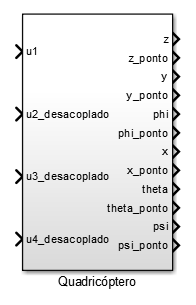
\includegraphics[width=0.3\textwidth]{./04-figuras/figuras_pos_banca/1-mostrando_desacoplamento/diagram_drone_block}
    \label{fig:diagram_drone_block}
\end{figure}

\section{Controladores Fuzzy}
\label{sec:controlador-fuzzy}

O projeto dos controlador \textit{fuzzy} foi focado na estabilização de atitude e altitude de um \textit{drone} sujeito a parâmetros específicos\footnote{Estes valores foram também utilizados por \citeonline{Balas2007} para definir uma especificação do sistema}, sendo eles: a gravidade $g=9,81$ m/s\textsuperscript{2}, a massa do quadricóptero $m=2,3$ kg e o comprimento de cada haste do \textit{drone} $l=0,5$ m. Um dos controladores projetado tem, como objetivo, controlar a altitude do quadricóptero, ao passo que um segundo visa a sua estabilização de sua atitude.

O controlador de altitude possui duas entradas e uma saída. As entradas são referentes à posição vertical do quadricóptero ($z$) e sua respectiva velocidade ($\dot{z}$), ao passo que a saída diz respeito ao sinal de controle a ser aplicado sobre o sistema para estabilizar sua altitude ($u_1$). Sua aplicação no sistema é mostrada na Figura \ref{fig:u1_mamdani_blocks}.

% Mostrar diagrama do sistema controlado (para ruídos), sobre a entrada u1
\begin{figure}[!htb]
    \centering
    \caption{Diagrama do sistema de controle de altitude utilizando controlador fuzzy}
    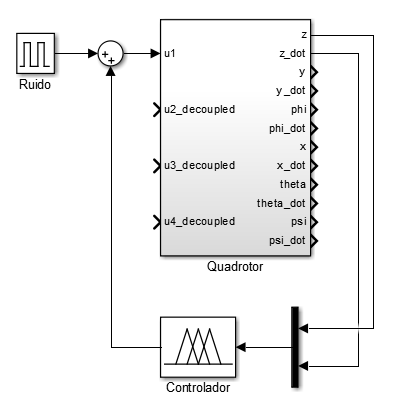
\includegraphics[width=0.5\textwidth]{./04-figuras/resultados/novos/simulink_printscreen_z}
    \label{fig:u1_mamdani_blocks}
\end{figure}

Utilizando o \textit{Fuzzy Logic Toolbox} do MATLAB, cada variável linguística do controlador fuzzy foi divida em três conjuntos: N (negativo), Z (zero) e P (positivo), tomando como base os trabalhos de \citeonline{Maj2013} e \citeonline{Gao2014Stability}. As regras fuzzy definidas para este controlador são mostradas no Quadro \ref{qua:regras_fuzzy_u1_mamdani}, e a Figura \ref{fig:1_mamdani_surface} exibe seu equivalente em superfície.

% Mostrar regras Fuzzy envolvidas no controle de u1 (quadro de regras + superfície)
% Tá errada!
\begin{quadro}[!htb]
    \centering
    \caption{Regras fuzzy para modelagem do controle de altitude\label{qua:regras_fuzzy_u1_mamdani}}
    \begin{tabular}{|c|c|c|}
    % \begin{tabular}{>{\centering\bfseries}m{1in} >{\centering}m{1in}
        \hline
        \textbf{{$z$}} & 
        \textbf{{$\dot{z}$}} &
        \textbf{{$u_1$}} \\
        \hline %01
            N &
            - &
            N \\
        \hline %02
            P &
            - &
            P \\
        \hline %03
            Z &
            N &
            N \\
        \hline %04
            Z &
            Z &
            Z \\
        \hline %05
            Z &
            P &
            P \\
        \hline
    \end{tabular}
    % \begin{TAB}(r,1cm,2cm)[5pt]{|c|c|}{|c|c|c|}% (rows,min,max)[tabcolsep]{columns}{rows}
    %     hi & tall one    \\
    %     hi & medium one  \\
    %     hi & standard one\\
    % \end{TAB}
\end{quadro}


\begin{figure}[!htb]
    \centering
    \caption{Superfície das regras do sistema de controle fuzzy para a altitude do quadrotor}
    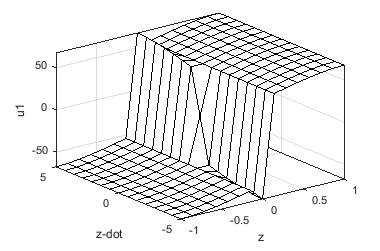
\includegraphics[width=0.6\textwidth]{./04-figuras/resultados/fis_u1/u1_mamdani_surface}
    \label{fig:1_mamdani_surface}
\end{figure}

O controlador de atitude projetado também possui duas entradas e uma saída. Desta vez, entretanto, as entradas são referentes ao ângulo em relação ao eixo horizontal ($\phi$ ou $\theta$) e sua respectiva variação ($\dot{\phi}$ ou $\dot{\theta}$). Mais uma vez, cada variável linguística foi dividida em três conjuntos: N, Z e P.

As regras que regem o controlador de atitude são sintetizadas no Quadro \ref{qua:regras_fuzzy_u2_u3_mamdani} e podem ser vistas na superfície de regras mostradas na Figura \ref{fig:u2_u3_mamdani_surface}.

% Mostrar regras Fuzzy envolvidas no controle de u2 e u3 (quadro de regras + superfície)
\begin{quadro}[!htb]
    \centering
    \caption{Regras fuzzy para modelagem do controle de atitude\label{qua:regras_fuzzy_u2_u3_mamdani}}
    \begin{tabular}{|c|c|c|}
    % \begin{tabular}{>{\centering\bfseries}m{1in} >{\centering}m{1in}
        \hline
        \textbf{{$\phi/\theta$}} & 
        \textbf{{$\dot{\phi}/\dot{\theta}$}} &
        \textbf{{$u_2/u_3$}} \\
        \hline %01
            P &
            P &
            N \\
        \hline %02
            P &
            Z &
            N \\
        \hline %03
            P &
            N &
            Z \\
        \hline %04
            N &
            N &
            P \\
        \hline %05
            N &
            Z &
            P \\
        \hline %06
            N &
            P &
            Z \\
        \hline %07
            Z &
            Z &
            Z \\
        \hline %08
            Z &
            N &
            P \\
        \hline %09
            Z &
            P &
            N \\
        \hline
    \end{tabular}
    % \begin{TAB}(r,1cm,2cm)[5pt]{|c|c|}{|c|c|c|}% (rows,min,max)[tabcolsep]{columns}{rows}
    %     hi & tall one    \\
    %     hi & medium one  \\
    %     hi & standard one\\
    % \end{TAB}
\end{quadro}


\begin{figure}[!htb]
    \centering
    \caption{Superfície das regras do sistema de controle fuzzy para a atitude do quadrotor}
    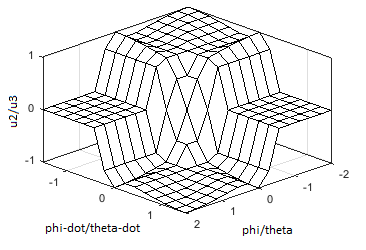
\includegraphics[width=0.6\textwidth]{./04-figuras/resultados/fis_u2/u2_u3_mamdani_surface}
    \label{fig:u2_u3_mamdani_surface}
\end{figure}

Já as Figuras \ref{fig:u2_mamdani_blocks} e \ref{fig:u3_mamdani_blocks} exibem os diagramas do sistema controlado, com atuação sobre os ângulos $\phi$ e $\theta$, respectivamente.

% Mostrar diagrama do sistema controlado (para ruídos), sobre as entradas u2 e u3
\begin{figure}[!htb]
    \centering
    \caption{Diagrama do sistema de controle de atitude utilizando controlador fuzzy sobre o ângulo $\phi$}
    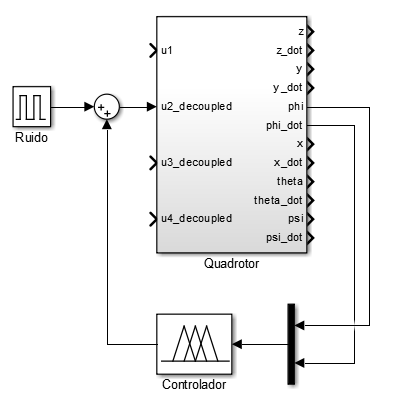
\includegraphics[width=0.6\textwidth]{./04-figuras/resultados/novos/simulink_printscreen_phi}
    \label{fig:u2_mamdani_blocks}
\end{figure}

\begin{figure}[!htb]
    \centering
    \caption{Diagrama do sistema de controle de atitude utilizando controlador fuzzy sobre o ângulo $\theta$}
    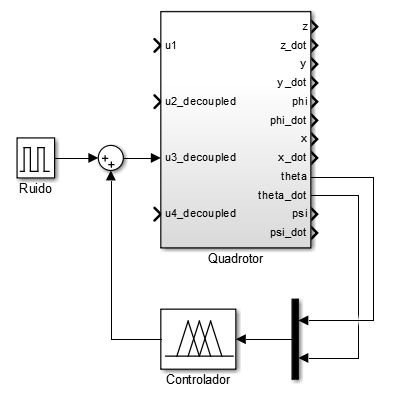
\includegraphics[width=0.5\textwidth]{./04-figuras/resultados/novos/simulink_printscreen_theta}
    \label{fig:u3_mamdani_blocks}
\end{figure}









\section{Controladores Neuro-Fuzzy}
\label{sec:controlador-neuro-fuzzy}

A partir dos controladores de atitude e altitude \textit{fuzzy} projetados, foram propostos dois controladores do tipo neuro-\textit{fuzzy}: um para cada dos casos.

Para tanto, foram utilizados os códigos mostrados nos Apêndices \ref{chap:train-anfis-altitude} e \ref{chap:train-anfis-atitude}. No processo de criação do controlador de altitude neuro-\textit{fuzzy}, foram gerados trezentos\footnote{Este valor foi arbitrado por corresponder a uma quantidade razoável para treinar a RNA sem que se alcance o sobre-parametrização, conhecido como \textit{overfitting}.} pares de entradas e cada um deles foi submetido ao processo de inferência \textit{fuzzy} utilizando o controlador previamente modelado e descrito na Seção \ref{sec:controlador-fuzzy}. Dois terços desses dados foram utilizados para gerar o conjunto de treinamento, representado pela variável {\ttfamily train} e o um terço restante foi armazenado na variável {\ttfamily test} e utilizado para validação do treinamento. Então, utilizando o comando {\ttfamily mam2sug} do MATLAB, foi gerado um modelo fuzzy Sugeno a partir do Mamdani que havia sido modelado e este novo arquivo foi salvo sob o nome {\ttfamily fis\_altitude\_neuro.fis}.

Feito isto, utilizou-se o comando comando {\ttfamily anfisedit} para abrir o \textit{Neuro-Fuzzy Designer} do MATLAB, cuja interface é mostrada na Figura \ref{fig:anfisedit_screen}. No campo marcado pelo número 2 na imagem (\textit{Generate FIS}), clicou-se no botão \textit{Load} e se selecionou o arquivo {\ttfamily fis\_altitude\_neuro.fis} que fora gerado pelo código executado. Após isto, no campo marcado pelo número 1 (\textit{Load Data}), marcou-se \textit{Training} e \textit{worksp} para utilizar uma variável da área de trabalho do MATLAB para treinar a rede. Após clicar em \textit{Load Data}, digitou-se {\ttfamily train}, nome da variável definida no código. Então, no campo marcado pelo número 3, marcou-se \textit{Training Data} e se clicou no botão \textit{Test Now} para executar o treinamento da rede. Após estes passos, a rede neuro-fuzzy foi devidamente treinada e sua estrutura, mostrada na Figura \ref{fig:rna_anfis_altitude_gray}, pode ser obtida clicando no botão \textit{Structure} logo acima do campo 3. Esta estrutura relaciona as variáveis de entrada e suas funções de pertinência, através das regras fuzzy, à saída do sistema e às suas funções de pertinência, em que cada componente representa um neurônio da RNA obtida. 

\begin{figure}[!htb]
    \centering
    \caption{Interface gráfica da ferramenta \textit{Neuro-Fuzzy Designer} com destaque aos três campos necessários para treinamento e teste da rede neuro-fuzzy}
    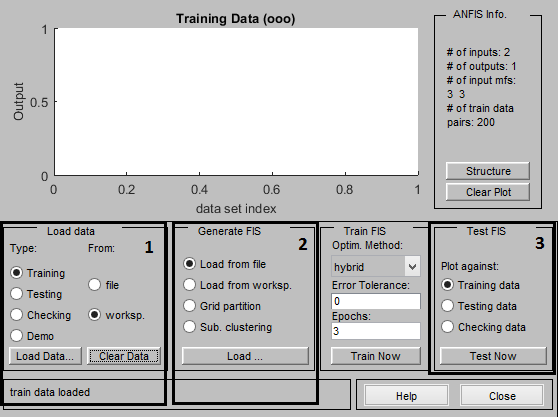
\includegraphics[width=0.8\textwidth]{./04-figuras/anfisedit/anfisedit_screen}
    \label{fig:anfisedit_screen}
\end{figure}

\begin{figure}[!htb]
    \centering
    \caption{Diagrama da RNA referente ao controlador neuro-fuzzy para altitude}
    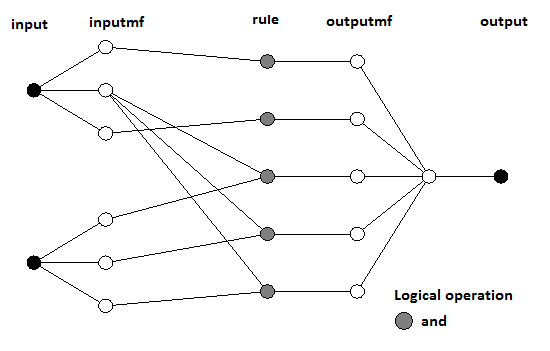
\includegraphics[width=0.6\textwidth]{./04-figuras/anfisedit/rna_anfis_altitude_gray}
    \label{fig:rna_anfis_altitude_gray}
\end{figure}

Após o término do treinamento, deve-se submeter a rede ao processo de teste. Para tanto, basta selecionar \textit{Testing} no campo marcado pelo número 1, deixar marcada a opção \textit{workspace}, clicar no botão \textit{Load Data} e escolher a variável {\ttfamily test}, que também foi definida no código executado.

A Figura \ref{fig:rna_anfis_train_result_altitude} mostra o gráfico obtido na ferramenta após o processo de treinamento, em que os círculos brancos mostram os dados utilizados no treinamento e os asteriscos pretos indicam o valor referentes a eles obtidos pela rede treinada.

\begin{figure}[!htb]
    \centering
    \caption{Resultado obtido pelo treinamento da RNA para controle de altitude}
    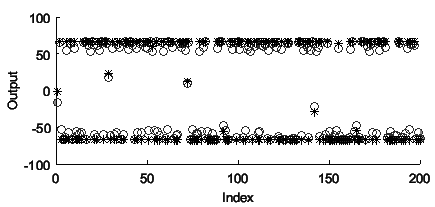
\includegraphics[width=0.6\textwidth]{./04-figuras/anfisedit/rna_anfis_train_result_altitude}
    \label{fig:rna_anfis_train_result_altitude}
\end{figure}

%Feito isto, após utilizar o comando {\ttfamily anfisedit} para abrir o \textit{Neuro-Fuzzy Designer} do MATLAB, carregou-se, nesta ferramenta, o arquivo {\ttfamily fis\_altitude\_neuro.fis} como sistema a ser treinado e, utilizando as variáveis {\ttfamily train} e {\ttfamily test}, o sistema foi devidamente treinado e validado. Após este processo, obteve-se um controlador neuro-fuzzy cujo funcionamento é mostrado pela superfície de regras mostradas na Figura \ref{fig:u1_sugeno_surface}.

Um processo similar foi aplicado para modelar o controlador de atitude neuro-fuzzy, como mostra o Apêndice \ref{chap:train-anfis-atitude}. As Figuras \ref{fig:rna_anfis_atitude_gray} e \ref{fig:rna_anfis_train_result_atitude} mostram o diagrama da RNA referente ao controlador neuro-fuzzy para atitude e o resultado obtido pelo seu treinamento respectivamente.

\begin{figure}[!htb]
    \centering
    \caption{Diagrama da RNA referente ao controlador neuro-fuzzy para atitude}
    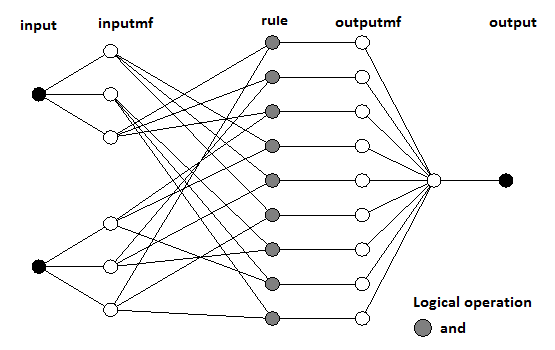
\includegraphics[width=0.6\textwidth]{./04-figuras/anfisedit/rna_anfis_atitude_gray}
    \label{fig:rna_anfis_atitude_gray}
\end{figure}

\begin{figure}[!htb]
    \centering
    \caption{Resultado obtido pelo treinamento da RNA para controle de atitude}
    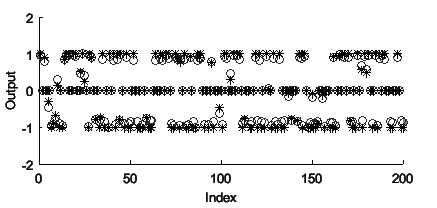
\includegraphics[width=0.6\textwidth]{./04-figuras/anfisedit/rna_anfis_train_result_atitude}
    \label{fig:rna_anfis_train_result_atitude}
\end{figure}

O processo de treinamento determina o comportamento dos controladores neuro-fuzzy projetados, cujas superfícies de regras são exibidas nas Figuras \ref{fig:u1_sugeno_surface} e \ref{fig:u2_u3_sugeno_surface}.

%-----
%Utilizando o comando {\ttfamily mam2sug} do MATLAB, obteve-se um novo modelo fuzzy do tipo Sugeno para cada modelo previamente definidos: um para controle de altitude e um segundo para controle de atitude do quadrotor. Então, utilizando o \textit{Neuro-Fuzzy Designer} do MATLAB, cada um dos modelos Sugeno criados foi treinado a partir de resultados obtidos pelos modelos fuzzy previamente elaborados. Não houve nenhuma alteração nas regras dos sistema, mas, devido às generalizações e aprendizagem da rede neuro-fuzzy, a relação entre valores de cada conjunto de saída foi ligeiramente alterado. Isso pode ser visto a partir das superfícies de regras para ambos os controladores, mostradas nas Figuras \ref{fig:u1_sugeno_surface} e \ref{fig:u2_u3_sugeno_surface}.

% Mostrar superfície Sugeno
\begin{figure}[!htb]
    \centering
    \caption{Superfície das regras do sistema de controle neuro-fuzzy para a altitude do quadrotor}
    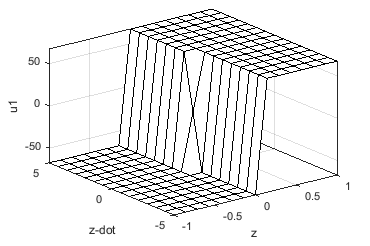
\includegraphics[width=0.6\textwidth]{./04-figuras/resultados/fis_u1/u1_sugeno_surface}
    \label{fig:u1_sugeno_surface}
\end{figure}

\begin{figure}[!htb]
    \centering
    \caption{Superfície das regras do sistema de controle fuzzy para a atitude do quadrotor}
    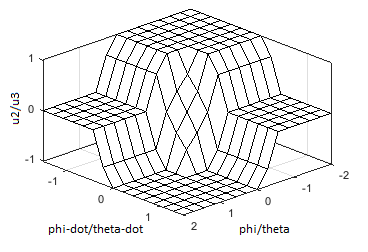
\includegraphics[width=0.6\textwidth]{./04-figuras/resultados/fis_u3/u2_u3_sugeno_surface}
    \label{fig:u2_u3_sugeno_surface}
\end{figure}




\section{Experimentos Realizados}
\label{sec:experimentos-realizados}
%O primeiro experimento feito foi para mostrar a instabilidade do sistema, mostrando a resposta das variáveis relacionadas à atitude (ângulos $\phi$ e $\theta$) e altitude ($z$) quando o sistema é submetido a um breve impulso em suas entradas, simulando qualquer força que possa atuar brevemente sobre o quadrotor, como um golpe sofrido por qualquer objeto que colida com ele. Após contextualizada a necessidade de controladores, passou-se à sua implementação e uso.

Uma vez projetados os controladores \textit{fuzzy} e neuro-\textit{fuzzy}, o sistema foi sujeitado a distúrbios em pulso em atitude e altitude para verificar o funcionamento deles sob condições similares às mostradas quando nenhum controle agia sobre ele fazendo com que o sistema divergisse. Primeiramente, o comportamento de ambos os controladores foi verificado quando atuando sobre o sistema para os quais eles foram projetados, com $g=9,81$ m/s\textsuperscript{2}, $m=2,3$ kg e $l=0,5$ m. 

Em seguida, para testar a robustez de cada controlador, foi feita uma simulação em que eles atuam sobre um sistema cuja massa do quadricóptero é $m=5$ kg, valor este que foi escolhido por variar o parâmetro massa em mais de 100 \%.

Por fim, foi testado o funcionamento do sistema quando um ruído de medição passa a fazer parte dele. Para tanto, um sinal aleatório de ruído foi somado ao valor real obtido de $z$, como mostrado na Figura \ref{fig:diagrama_sistema_com_ruido}.

\begin{figure}[!htb]
    \centering
    \caption{Representação do quadricóptero no \textit{Simulink} na simulação envolvendo ruído de medição de $z$}
    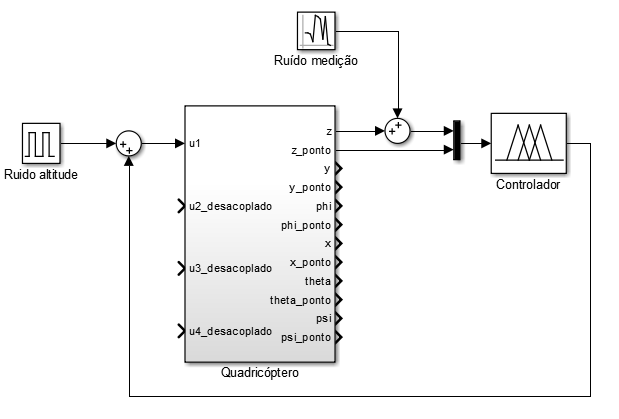
\includegraphics[width=1\textwidth]{./04-figuras/figuras_pos_banca/7-altitude2kg_ruido/diagrama_sistema_com_ruido}
    \label{fig:diagrama_sistema_com_ruido}
\end{figure}

Os resultados obtidos são mostrados no capítulo seguinte.